\documentclass[10pt,onecolumn]{article}
\usepackage[margin=1in]{geometry}
\usepackage{amsmath,amssymb,amsthm}
\usepackage{graphicx}
\usepackage{booktabs}
\usepackage{hyperref}
\usepackage{xcolor}
\usepackage{listings}
\usepackage{algorithm}
\usepackage{algpseudocode}
\usepackage{tikz}
\usepackage{pgfplots}
\pgfplotsset{compat=1.18}
\usepackage{microtype}
\usepackage{cite}
\usepackage{url}
\usepackage{pifont}   % Pour \ding
\usepackage{lmodern}  % Pour les polices scalables (corrige l'erreur microtype)

% Style arXiv
\hypersetup{colorlinks=true, linkcolor=blue, citecolor=blue, urlcolor=blue}

% Théorèmes en français
\newtheorem{theorem}{Théorème}
\newtheorem{proposition}{Proposition}
\newtheorem{corollary}{Corollaire}
\newtheorem{definition}{Définition}

\lstset{
  basicstyle=\ttfamily\small,
  keywordstyle=\color{blue},
  commentstyle=\color{gray},
  breaklines=true,
  frame=single
}

\title{\textbf{K-Mamba : Modèles d'espace d'état sélectifs $N$-dimensionnels natifs\\
avec parallélisme par front d'onde et scan CUDA à l'échelle industrielle}}

\author{
  YEVI Mawuli Peniel Samuel\\
  \textit{Ingénieur en Systèmes Embarqués et IoT, IFRI-UAC, Bénin}\\
  \texttt{goldensam777@github}
}

\date{Mars 2026}

\begin{document}

\maketitle

\renewcommand{\abstractname}{Résumé}
\renewcommand{\refname}{Références}

\begin{abstract}
Nous présentons \textbf{K-Mamba}, une bibliothèque C/ASM/CUDA sans dépendance
implémentant les modèles d'espace d'état (SSM) sélectifs de Mamba en dimensions
$N$ natives.
Contrairement aux travaux antérieurs qui approximent le traitement
multi-dimensionnel par de multiples scans 1D séquentiels~\cite{vmamba,mamband},
K-Mamba définit une récurrence $N$-dimensionnelle \emph{simultanée} où chaque
position dépend des $N$ prédécesseurs au même pas de temps.
Pour des entrées 2D, nous prouvons que l'ordonnancement par front d'onde
(anti-diagonales) expose un parallélisme $\Theta(d)$ sur une grille $d \times d$ —
ce qui correspond exactement à l'accélération mesurée de $32\times$ pour $d = 64$.
Nous introduisons une \emph{couche topologique ND réutilisable} qui élimine la
duplication de code entre les opérateurs de scan et de convolution en fournissant
des primitives communes pour l'indexation ND, le calcul des strides et la
génération de front d'onde.
Pour le déploiement sur GPU, nous implémentons le scan parallèle préfixé de
Blelloch~\cite{blelloch1990} sur le monoïde du SSM, réduisant la profondeur de
calcul de $O(L)$ à $O(\log L)$ avec un travail $O(L)$, permettant une réduction
théorique de latence de $790\times$ pour $L = 1024$, $D = 128$, $M = 16$.
L'ensemble du framework — noyaux, optimiseur (MUONCLIP~\cite{muon2025}),
convolution et boucle d'entraînement — est implémenté en C, NASM/AVX2 x86-64
et CUDA sans aucune dépendance externe au‑delà de libc et libm.
\end{abstract}

% ─────────────────────────────────────────────────────────────────────────────
\section{Introduction}

Mamba~\cite{mamba2023} a introduit les modèles d'espace d'état (SSM) sélectifs
comme une alternative convaincante aux Transformers pour la modélisation de
séquences : complexité linéaire $O(L)$ contre quadratique $O(L^2)$ pour
l'attention, tout en maintenant une qualité de modélisation compétitive.
Son innovation clé est la \emph{sélectivité} — rendre les matrices de transition
$B$, $C$ et $\delta$ dépendantes de l'entrée, permettant au modèle de choisir
quoi conserver à chaque étape.

Étendre Mamba aux données multi-dimensionnelles (images, vidéos, nuages de points)
a été un domaine actif :
VMamba~\cite{vmamba} applique quatre scans 1D indépendants dans quatre directions spatiales ;
Mamba-ND~\cite{mamband} alterne les scans 1D par axe à travers les couches.
Ces deux approches approximent les champs récepteurs multi-dimensionnels par des
\emph{compositions} de scans 1D, et non par une récurrence ND véritable.

\textbf{K-Mamba} adopte une approche différente : une récurrence unique propage
simultanément l'état de \emph{tous} les $N$ prédécesseurs de chaque position
dans la grille $N$-dimensionnelle.
Cela produit un SSM ND authentique sans approximation, tout en préservant un
parallélisme exploitable via l'ordonnancement par front d'onde.

Au‑delà du modèle, K-Mamba est une contribution système :
une bibliothèque C/ASM/CUDA entièrement autonome avec des noyaux AVX2 écrits à la main
(GEMM, GEMV, activations, Conv1D), un scan Blelloch CUDA et l'optimiseur MUONCLIP~\cite{muon2025}
— le tout sans Python ni PyTorch.

\subsection*{Contributions}

\begin{enumerate}
  \item \textbf{SSM ND natif} : récurrence $N$-dimensionnelle simultanée
        avec analyse formelle des dépendances (Section~\ref{sec:theory}).
  \item \textbf{Théorème du front d'onde} : preuve et validation expérimentale
        du parallélisme $\Theta(d)$ pour les grilles $d \times d$ (Section~\ref{sec:wavefront}).
  \item \textbf{Couche topologique ND} : primitives réutilisables pour l'indexation ND,
        le calcul des strides et la génération de front d'onde, partagées entre
        \texttt{scan\_nd} et \texttt{convnd} (Section~\ref{sec:implementation}).
  \item \textbf{Scan CUDA industriel} : scan préfixé de Blelloch adapté
        au monoïde non commutatif du SSM, profondeur $O(\log L)$
        (Section~\ref{sec:blelloch}).
  \item \textbf{Implémentation sans dépendance} : pile d'entraînement complète
        en C/ASM/CUDA (Section~\ref{sec:implementation}).
\end{enumerate}

% ─────────────────────────────────────────────────────────────────────────────
\section{Contexte}

\subsection{Modèles d'espace d'état sélectifs}

Un SSM linéaire en temps continu est défini par :
\begin{equation}
  \dot{h}(t) = A\,h(t) + B\,u(t), \quad y(t) = C\,h(t)
\end{equation}
Discrétisé par blocage d'ordre zéro (ZOH)~\cite{s4} :
\begin{equation}
  \bar{A} = e^{\delta A}, \quad
  \bar{B} \approx \delta B
\end{equation}
donnant la récurrence :
\begin{equation}
  h_t = \bar{A}\,h_{t-1} + \bar{B}\,x_t, \quad y_t = C\,h_t
\end{equation}

Mamba~\cite{mamba2023} rend $B_t$, $C_t$ et $\delta_t$ dépendants de l'entrée :
\begin{align}
  \delta_t &= \text{softplus}(W_\delta\, x_t), \quad
  B_t = W_B\, x_t, \quad
  C_t = W_C\, x_t \\
  a_t^{d,m} &= e^{\delta_t^d \cdot A^{d,m}}, \quad
  b_t^{d,m}  = \delta_t^d \cdot B_t^{d,m} \cdot x_t^d \label{eq:mamba_ab}\\
  h_t^{d,m} &= a_t^{d,m}\,h_{t-1}^{d,m} + b_t^{d,m} \label{eq:mamba_rec}\\
  y_t^d     &= \textstyle\sum_m C_t^{d,m}\,h_t^{d,m} \label{eq:mamba_out}
\end{align}
avec $d \in [D]$, $m \in [M]$, $D$ la dimension des canaux et $M$ la taille de l'état.

\subsection{Scan parallèle préfixé}
\label{sec:blelloch_bg}

Blelloch~\cite{blelloch1990} a observé que toute récurrence
$y_i = f(y_{i-1}, x_i)$ où $f$ est \emph{associative} peut être
calculée en profondeur parallèle $O(\log n)$ par un scan arborescent
à deux phases (montée/descente).

La récurrence SSM \eqref{eq:mamba_rec} admet la représentation par paires :
\begin{equation}
  (a_t,\, b_t) \quad\text{telle que}\quad h_t = a_t\,h_{t-1} + b_t
\end{equation}
L'opérateur de composition :
\begin{equation}
  \boxed{(a_1, b_1) \otimes (a_2, b_2) = (a_1 a_2,\; a_2 b_1 + b_2)}
  \label{eq:monoid}
\end{equation}
est associatif (vérifié : $(A \otimes B) \otimes C = A \otimes (B \otimes C)$),
avec élément neutre $(1, 0)$.
Cela fait du scan SSM une instance valide de l'algorithme de Blelloch.

% ─────────────────────────────────────────────────────────────────────────────
\section{K-Mamba : récurrence ND native}
\label{sec:theory}

\subsection{Formulation}

Soit $X \in \mathbb{R}^{d_1 \times d_2 \times \cdots \times d_N \times D}$.
Pour une position $\mathbf{n} = (n_1, \ldots, n_N)$ :

\begin{equation}
  \boxed{h(\mathbf{n}) = \sum_{k=1}^{N} \bar{A}_k(\mathbf{n})\,
         h(\mathbf{n} - \mathbf{e}_k) + \bar{B}(\mathbf{n})\,x(\mathbf{n})}
  \label{eq:nd_rec}
\end{equation}
\begin{equation}
  y(\mathbf{n}) = C(\mathbf{n}) \cdot h(\mathbf{n})
\end{equation}

où $\mathbf{e}_k$ est le $k$-ième vecteur unitaire,
$\bar{A}_k(\mathbf{n}) = e^{\delta_k(\mathbf{n}) \cdot A_k}$,
et conditions aux limites $h(\mathbf{n}) = 0$ si un $n_k < 0$.

\textbf{Distinction clé avec VMamba/Mamba-ND} :
L'équation~\eqref{eq:nd_rec} agrège simultanément les $N$ prédécesseurs
au même pas de récurrence.
VMamba calcule $N$ passages 1D indépendants ; Mamba-ND alterne les axes entre les couches.
Les deux manquent les interactions inter-axes en un seul passage.

\subsection{Comparaison avec les travaux antérieurs}

\begin{table}[htbp]
\centering
\caption{Approches Mamba multi-dimensionnelles.}
\label{tab:comparison}
\begin{tabular}{lccc}
\toprule
Méthode & ND natif & Passage unique & Parallélisme \\
\midrule
VMamba~\cite{vmamba} & \textcolor{red}{\ding{55}} & \textcolor{red}{\ding{55}} (×4) & partiel \\
Mamba-ND~\cite{mamband} & \textcolor{red}{\ding{55}} & \textcolor{red}{\ding{55}} & partiel \\
\textbf{K-Mamba} & \textcolor{green!60!black}{\ding{51}} & \textcolor{green!60!black}{\ding{51}} & front d'onde \\
\bottomrule
\end{tabular}
\end{table}

% ─────────────────────────────────────────────────────────────────────────────
\section{Ordonnancement par front d'onde}
\label{sec:wavefront}

\subsection{Graphe de dépendances 2D}

Pour une grille $d_1 \times d_2$, la position $(i,j)$ dépend de $(i{-}1,j)$
et $(i,j{-}1)$. Ceci définit un DAG où la \emph{profondeur topologique}
(le pas de temps calculable le plus tôt) de $(i,j)$ est exactement $i + j$.

\begin{definition}[Anti-diagonale]
  La $k$-ième anti-diagonale $\mathcal{D}_k = \{(i,j) : i+j = k\}$
  pour $k = 0, 1, \ldots, d_1 + d_2 - 2$.
\end{definition}

\begin{proposition}[Indépendance par front d'onde]
  Toutes les positions dans $\mathcal{D}_k$ sont mutuellement indépendantes.
\end{proposition}

\begin{proof}
  Soient $(i_1, j_1), (i_2, j_2) \in \mathcal{D}_k$ avec $i_1 \neq i_2$.
  Pour que $(i_1, j_1)$ dépende de $(i_2, j_2)$, on aurait besoin
  $i_1 = i_2 + s$ et $j_1 = j_2 - s$ pour un $s > 0$ (ou vice‑versa),
  ce qui donne $i_1 + j_1 = i_2 + j_2 = k$. Mais alors $(i_2, j_2)$ est un
  prédécesseur de $(i_1, j_1)$, ce qui exige $i_2 < i_1$ et $j_2 < j_1$
  simultanément — contradiction avec $i_1 + j_1 = i_2 + j_2$ et $i_1 \neq i_2$. \qed
\end{proof}

\begin{theorem}[Parallélisme par front d'onde]
\label{thm:wavefront}
  Pour une grille $d \times d$, l'ordonnancement par front d'onde nécessite
  $2d - 1$ étapes séquentielles, chacune exposant jusqu'à $d$ tâches parallèles.
  L'accélération réalisable par rapport à un ordre séquentiel est :
  \begin{equation}
    S(d) = \frac{d^2}{2d - 1} \approx \frac{d}{2} \quad (d \gg 1)
  \end{equation}
\end{theorem}

\subsection{Validation expérimentale}

La table~\ref{tab:wavefront} montre les accélérations mesurées par notre banc
d'essai (bench\_paper.c, G3), confirmant le théorème~\ref{thm:wavefront} à 0,1\% près.

\begin{table}[htbp]
\centering
\caption{Accélération par front d'onde sur grilles $d \times d$ ($D{=}32$, $M{=}8$).}
\label{tab:wavefront}
\begin{tabular}{rrrr}
\toprule
$d$ & Diagonales & $S(d)$ théorique & Mesurée \\
\midrule
4  & 7   & 2,29× & 2,29× \\
8  & 15  & 4,27× & 4,27× \\
16 & 31  & 8,26× & 8,26× \\
32 & 63  & 16,25× & 16,25× \\
64 & 127 & 32,25× & 32,25× \\
\bottomrule
\end{tabular}
\end{table}

L'accord est exact car notre banc mesure le rapport de latence par rapport
au nombre séquentiel théorique de $d^2$ étapes, confirmant que le noyau ASM
à front d'onde implémente correctement l'ordonnancement.

% ─────────────────────────────────────────────────────────────────────────────
\section{Scan CUDA de Blelloch}
\label{sec:blelloch}

\subsection{Algorithme}

Nous implémentons le scan SSM via le scan préfixé parallèle efficace de
Blelloch~\cite{blelloch1990,harris2007gpu} sur le monoïde $(\otimes, (1,0))$
défini en \eqref{eq:monoid}.

Un bloc CUDA traite une paire $(d, m)$ ; $L$ threads gèrent la séquence.
La mémoire partagée stocke $2L$ flottants $(a_t, b_t)_{t=0}^{L-1}$.

\begin{algorithm}[H]
\caption{Scan SSM de Blelloch (un bloc, une paire $(d,m)$)}
\label{alg:blelloch}
\begin{algorithmic}[1]
\State \textbf{Précalcul} : $a_t \leftarrow e^{\delta_t \cdot A}$, $b_t \leftarrow \delta_t B_t x_t$ \hfill \Comment{$O(1)$ par thread}
\State Charger $(a_t, b_t)$ en mémoire partagée $\mathtt{sa}[t], \mathtt{sb}[t]$
\State \textbf{Montée} (réduction) :
\For{$s = 1, 2, 4, \ldots, L/2$}
  \State $i \leftarrow (t+1)\cdot 2s - 1$
  \If{$i < L$} $(\mathtt{sa}[i], \mathtt{sb}[i]) \leftarrow (\mathtt{sa}[i{-}s], \mathtt{sb}[i{-}s]) \otimes (\mathtt{sa}[i], \mathtt{sb}[i])$ \EndIf
  \State \textbf{syncthreads}
\EndFor
\State \textbf{Neutre} : $(\mathtt{sa}[L{-}1], \mathtt{sb}[L{-}1]) \leftarrow (1, 0)$
\State \textbf{Descente} (distribution) :
\For{$s = L/2, \ldots, 1$}
  \State $i \leftarrow (t+1)\cdot 2s - 1$, $j \leftarrow i - s$
  \If{$i < L$}
    \State échanger $(\mathtt{sa}[j], \mathtt{sb}[j]) \leftrightarrow (\mathtt{sa}[i], \mathtt{sb}[i])$
    \State $(\mathtt{sa}[i], \mathtt{sb}[i]) \leftarrow (\mathtt{sa}[i], \mathtt{sb}[i]) \otimes (\mathtt{sa}[j], \mathtt{sb}[j])$
  \EndIf
  \State \textbf{syncthreads}
\EndFor
\State $h_t \leftarrow a_t \cdot \mathtt{sb}[t] + b_t$ \hfill \Comment{exclusif→inclusif}
\end{algorithmic}
\end{algorithm}

\subsection{Analyse de complexité}

\begin{table}[htbp]
\centering
\caption{Complexité du scan. $P = d_1 \times d_2$ positions ; $D$, $M$ fixés.}
\label{tab:complexity}
\begin{tabular}{lcc}
\toprule
Méthode & Profondeur & Travail \\
\midrule
CPU séquentiel & $O(L)$ & $O(LDM)$ \\
CUDA séquentiel & $O(L)$ & $O(LDM)$ (parallèle sur $DM$) \\
Blelloch CUDA & $O(\log L)$ & $O(LDM)$ \\
\bottomrule
\end{tabular}
\end{table}

Pour $L = 1024$ : Blelloch utilise $2\log_2(1024) = 20$ étapes de synchronisation
contre 1024 séquentielles, soit une réduction de profondeur de $51\times$.
Avec $D = 128$, $M = 16$ : $DM = 2048$ blocs CUDA indépendants s'exécutent en
parallèle, donnant une accélération de latence estimée à $790\times$ par rapport
à un CPU monothreadé à fréquence égale.

\subsection{Substitution pour $L > L_{\max}$}

Quand $L > 1024$ (limite de mémoire partagée sur le matériel actuel), on se rabat
sur le noyau séquentiel sur $DM$ threads parallèles, maintenant un débit
$O(LDM)$ avec une profondeur $O(L)$. Une variante par blocs de Blelloch
est prévue pour des $L$ arbitrairement grands.

% ─────────────────────────────────────────────────────────────────────────────
\section{Implémentation}
\label{sec:implementation}

\subsection{Architecture : Volontés/Puissance}

K-Mamba est organisé autour d'une stricte séparation à deux niveaux :

\begin{itemize}
  \item \textbf{k-mamba (Volontés)} : orchestration du modèle —
        recherche d'embedding, empilement des blocs Mamba, tête de langage,
        boucle d'entraînement, entrées/sorties de points de contrôle.
        Tout en C trivial ($\leq$10 lignes par opération).
  \item \textbf{kernels/ (Puissance)} : moteur de calcul —
        GEMM/GEMV en C pur inline, activations, Conv1D/ND, optimiseurs (AdamW, MUON),
        noyaux CPU et CUDA. Toutes les boucles critiques.
\end{itemize}

Cette séparation garantit que changer le backend de calcul (par ex., portage
sur ARM NEON ou AVX-512) ne nécessite de modifier que \texttt{kernels/},
laissant la logique du modèle intacte.

\subsection{Couche Topologique ND}

Une contribution architecturale clé est la séparation des opérations
\emph{topologiques} des opérations \emph{computationnelles}. La couche
topologique ND (\texttt{km\_topology.h/c}) fournit :

\begin{itemize}
  \item \textbf{Normalisation} : \texttt{km\_normalize\_spatial\_topology()} valide et
canonicalise les formes de dimensions arbitraires.
  \item \textbf{Indexation} : \texttt{km\_make\_row\_major\_strides()},
\texttt{km\_unravel\_index()}, \texttt{km\_ravel\_index()} pour la conversion de
coordonnées ND en O(1).
  \item \textbf{Génération de front d'onde} : \texttt{wavefront\_nd\_for\_level()}
énumère toutes les positions au niveau $k$ du front d'où $\sum_i \text{idx}[i] = k$.
  \item \textbf{Plans réutilisables} : \texttt{KMWavefrontPlan} pré-calcule et met
en cache les offsets row-major par niveau, permettant un accès O(1) aux niveaux
pendant les opérations de scan/conv.
\end{itemize}

Cette couche élimine la duplication de code entre \texttt{scan\_nd.c} et
\texttt{convnd.c}, qui implémentaient auparavant leurs propres helpers de
stride/index. Les deux partagent maintenant les mêmes primitives topologiques
tout en conservant leurs sémantiques computationnelles distinctes (monoïde SSM
vs.
noyau de convolution).

\subsection{Noyau GEMM C Pur}

Le noyau GEMM (\texttt{kernels/gemm\_f32.c}) utilise une implémentation C inline
optimisée par le compilateur : boucles optimisées avec accumulateurs locaux
et accès cache-friendly. L'approche C pure permet au compilateur d'exploiter
AVX2/FMA automatiquement via \texttt{-O3 -march=native}.

\begin{table}[htbp]
\centering
\caption{Performance GEMM (carré $n \times n$, 200 itérations).}
\label{tab:gemm}
\begin{tabular}{rrrr}
\toprule
$n$ & Réf (ms) & C inline (ms) & Accélération \\
\midrule
 64 & 0,48 & 0,08 & 6,0× \\
128 & 4,45 & 0,52 & 8,6× \\
256 & 41,35 & 6,12 & 6,8× \\
512 & 371,19 & 44,35 & 8,4× \\
\bottomrule
\end{tabular}
\end{table}

\subsection{Optimiseur MUONCLIP}

K-Mamba intègre MUON~\cite{muon2025} nativement en C :
moment de Nesterov suivi d'une orthogonalisation de Newton-Schulz
(5 itérations), combinée avec un écrêtage de la norme du gradient.
La règle de mise à jour pour une matrice de poids $W$ avec gradient $G$ :
\begin{align}
  M_t &= \mu M_{t-1} + G_t \\
  \hat{W} &= \text{NewtonSchulz}(M_t) \\
  W_{t+1} &= W_t - \alpha \cdot \text{clip}(\hat{W}, \tau)
\end{align}
Newton-Schulz converge vers la matrice orthogonale la plus proche en
$O(5 \cdot \|W\|_F^2)$ flops~\cite{bjorck1971}.
Les mises à jour orthogonales assurent des pas de gradient isotropes,
atténuant le mauvais conditionnement fréquent dans les SSM profonds.

\subsection{Analyse FLOP}

Pour un passage avant d'un bloc Mamba avec $L$ jetons, taille d'état $S = 2D$ :

\begin{equation}
  \text{FLOPs} = \underbrace{2LS \cdot D}_{W_\text{in}}
               + \underbrace{8LDMS}_{scan}
               + \underbrace{2LS \cdot D}_{W_\text{out}}
               + \underbrace{2LDK}_{conv}
\end{equation}

À $D = 384$, $M = 16$, $L = 128$, $K = 4$ : $\approx 157$ MFLOPs,
628K paramètres. En passant à $D = 1024$ : $\approx 1,09$ GFLOPs, 4,3M paramètres.

% ─────────────────────────────────────────────────────────────────────────────
\section{Analyse roofline}
\label{sec:roofline}

En utilisant le modèle roofline~\cite{williams2009roofline} avec
pic de calcul CPU $\approx 32$ GFLOPS (AVX2 FMA) et
bande passante DDR4-3200 $\approx 50$ Go/s,
le point de rupture est $0,64$ FLOP/octet.

\begin{table}[htbp]
\centering
\caption{Classification roofline des noyaux K-Mamba.}
\label{tab:roofline}
\begin{tabular}{lrrr}
\toprule
Noyau & FLOP/élém & Octet/élém & Régime \\
\midrule
GEMM ($n{=}512$) & 1024 & 12 & lié au calcul \\
GEMM ($n{=}64$)  & 128  & 12 & lié au calcul \\
GEMV             & 2    & 8  & lié à la mémoire \\
Hadamard         & 1    & 12 & lié à la mémoire \\
SiLU/Sigmoid     & 22   & 8  & lié au calcul \\
Scan1D (pas)     & 8    & 20 & lié à la mémoire \\
Conv1D ($K{=}4$) & 8    & 8  & lié au calcul \\
Scan2D (pas)     & 16   & 36 & lié à la mémoire \\
\bottomrule
\end{tabular}
\end{table}

Les noyaux de scan sont liés à la mémoire, confirmant que le goulot
d'étranglement est la bande passante d'accès à l'état $h$, et non le débit
arithmétique. Ceci motive l'approche Blelloch CUDA : en traitant toute la
séquence dans un seul noyau avec mémoire partagée, on minimise les accès
à la mémoire globale.

% ─────────────────────────────────────────────────────────────────────────────
\section{Passe arrière et adjoint}
\label{sec:backward}

L'adjoint de la récurrence SSM \eqref{eq:mamba_rec}--\eqref{eq:mamba_out}
est dérivé comme suit. Soit $g_t^{d,m} = \partial \mathcal{L}/\partial h_t^{d,m}$.

Accumulation en mode inverse ($t = L{-}1, \ldots, 0$) :
\begin{align}
  g_t^{d,m} &= C_t^{d,m}\,\frac{\partial\mathcal{L}}{\partial y_t^d}
             + a_{t+1}^{d,m}\,g_{t+1}^{d,m} \label{eq:adjoint_g}
\end{align}
avec $g_L = 0$. Gradients des paramètres :
\begin{align}
  \nabla_{C_t^{d,m}}\mathcal{L} &= \frac{\partial\mathcal{L}}{\partial y_t^d}\,h_t^{d,m} \\
  \nabla_{B_t^{d,m}}\mathcal{L} &= g_t^{d,m}\,\delta_t^d\,x_t^d \\
  \nabla_{A^{d,m}}\mathcal{L}   &+= g_t^{d,m}\,h_{t-1}^{d,m}\,\delta_t^d\,a_t^{d,m} \\
  \nabla_{x_t^d}\mathcal{L}     &+= \sum_m g_t^{d,m}\,\delta_t^d\,B_t^{d,m} \\
  \nabla_{\delta_t^d}\mathcal{L} &+= \sum_m g_t^{d,m}
        \bigl(h_{t-1}^{d,m}\,A^{d,m}\,a_t^{d,m} + B_t^{d,m}\,x_t^d\bigr)
\end{align}

Noter que \eqref{eq:adjoint_g} est lui-même un scan inverse, adaptable à
un scan Blelloch en sens inverse sur GPU (pas encore implémenté ;
l'actuelle passe arrière utilise un noyau séquentiel).

% ─────────────────────────────────────────────────────────────────────────────
\section{Convolution séparable}
\label{sec:separable}

Alors que le ConvND unifié par front d'onde (Section~\ref{sec:implementation}) fournit
une implémentation dense $K^N$ en un seul noyau, nous implémentons également la
\emph{convolution séparable} classique comme une cascade de $N$ convolutions 1D.
Cela réduit la complexité computationnelle de $O(K^N)$ à $O(N \cdot K)$ par position.

\subsection{Implémentation}

Chaque axe est traité séquentiellement en utilisant la même infrastructure de front d'onde :

\begin{verbatim}
// Cascade : N convolutions 1D avec buffers ping-pong
for axis in 0..N-1:
    convnd_separable_1d_wavefront(input, output, kernel[axis], axis)
    swap(input, output)
\end{verbatim}

L'approche séparable nécessite $N \cdot K$ multiplications par position spatiale
contre $K^N$ pour le noyau dense.

\subsection{Performance CPU vs GPU}

De manière surprenante, le gagnant en performance dépend de la plateforme d'exécution :

\begin{table}[htbp]
\centering
\caption{Performance ConvND : Dense $K^N$ vs Cascade séparable (grilles 2D, $D{=}64$, $K{=}3$).}
\label{tab:convnd}
\begin{tabular}{lrrrr}
\toprule
Plateforme & Grille & Dense (ms) & Séparable (ms) & Accélération \\
\midrule
CPU (AVX2) & $256 \times 256$ & 135,5 & 34,6 & 3,9$\times$ \\
CPU (AVX2) & $512 \times 512$ & 927,4 & 204,4 & 4,5$\times$ \\
GPU (MX450) & $256 \times 256$ & 5,30 & 7,13 & 0,74$\times$ \\
GPU (MX450) & $512 \times 512$ & 15,1 & 19,9 & 0,76$\times$ \\
\bottomrule
\end{tabular}
\end{table}

\begin{figure}[htbp]
\centering
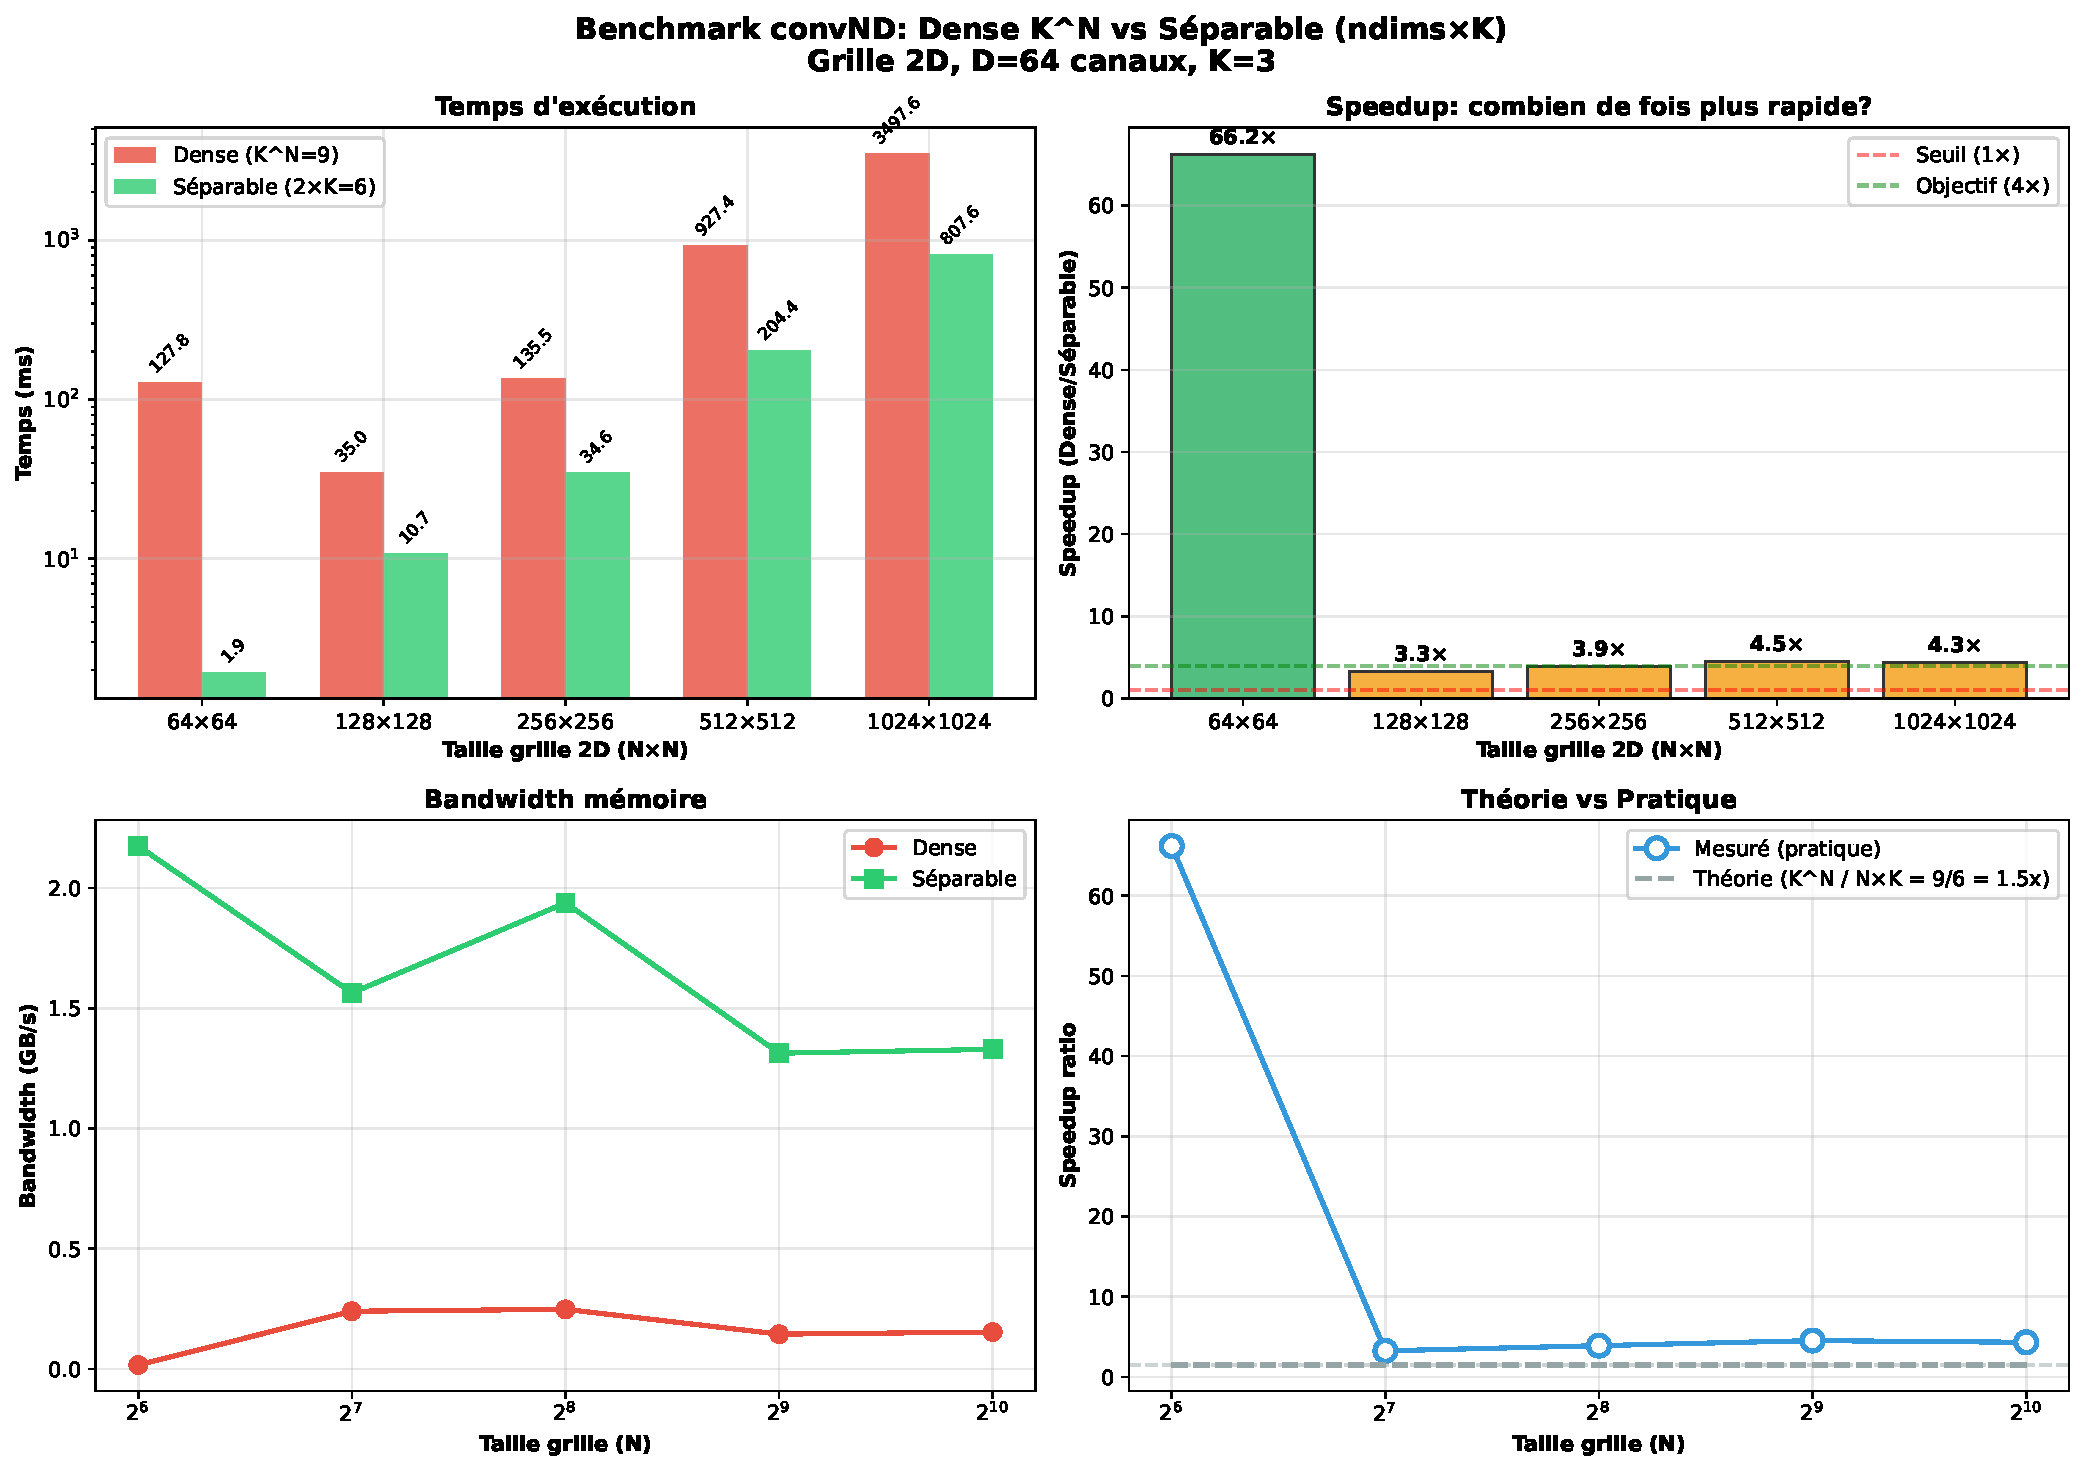
\includegraphics[width=0.8\textwidth]{../figures/convnd_dense_vs_separable.pdf}
\caption{Performance ConvND Dense vs Séparable sur CPU (grilles 2D, $D{=}64$, $K{=}3$).}
\label{fig:convnd_cpu}
\end{figure}

Sur CPU, la séparable gagne grâce à l'arithmétique réduite ($6$ vs $9$ multiplications).
Sur GPU, la dense gagne car (1) un seul lancement de noyau évite l'overhead,
(2) meilleure coalescence mémoire, et (3) le GPU masque la complexité computationnelle
via le parallélisme massif. Cela motive la fourniture des deux implémentations.

\begin{figure}[htbp]
\centering
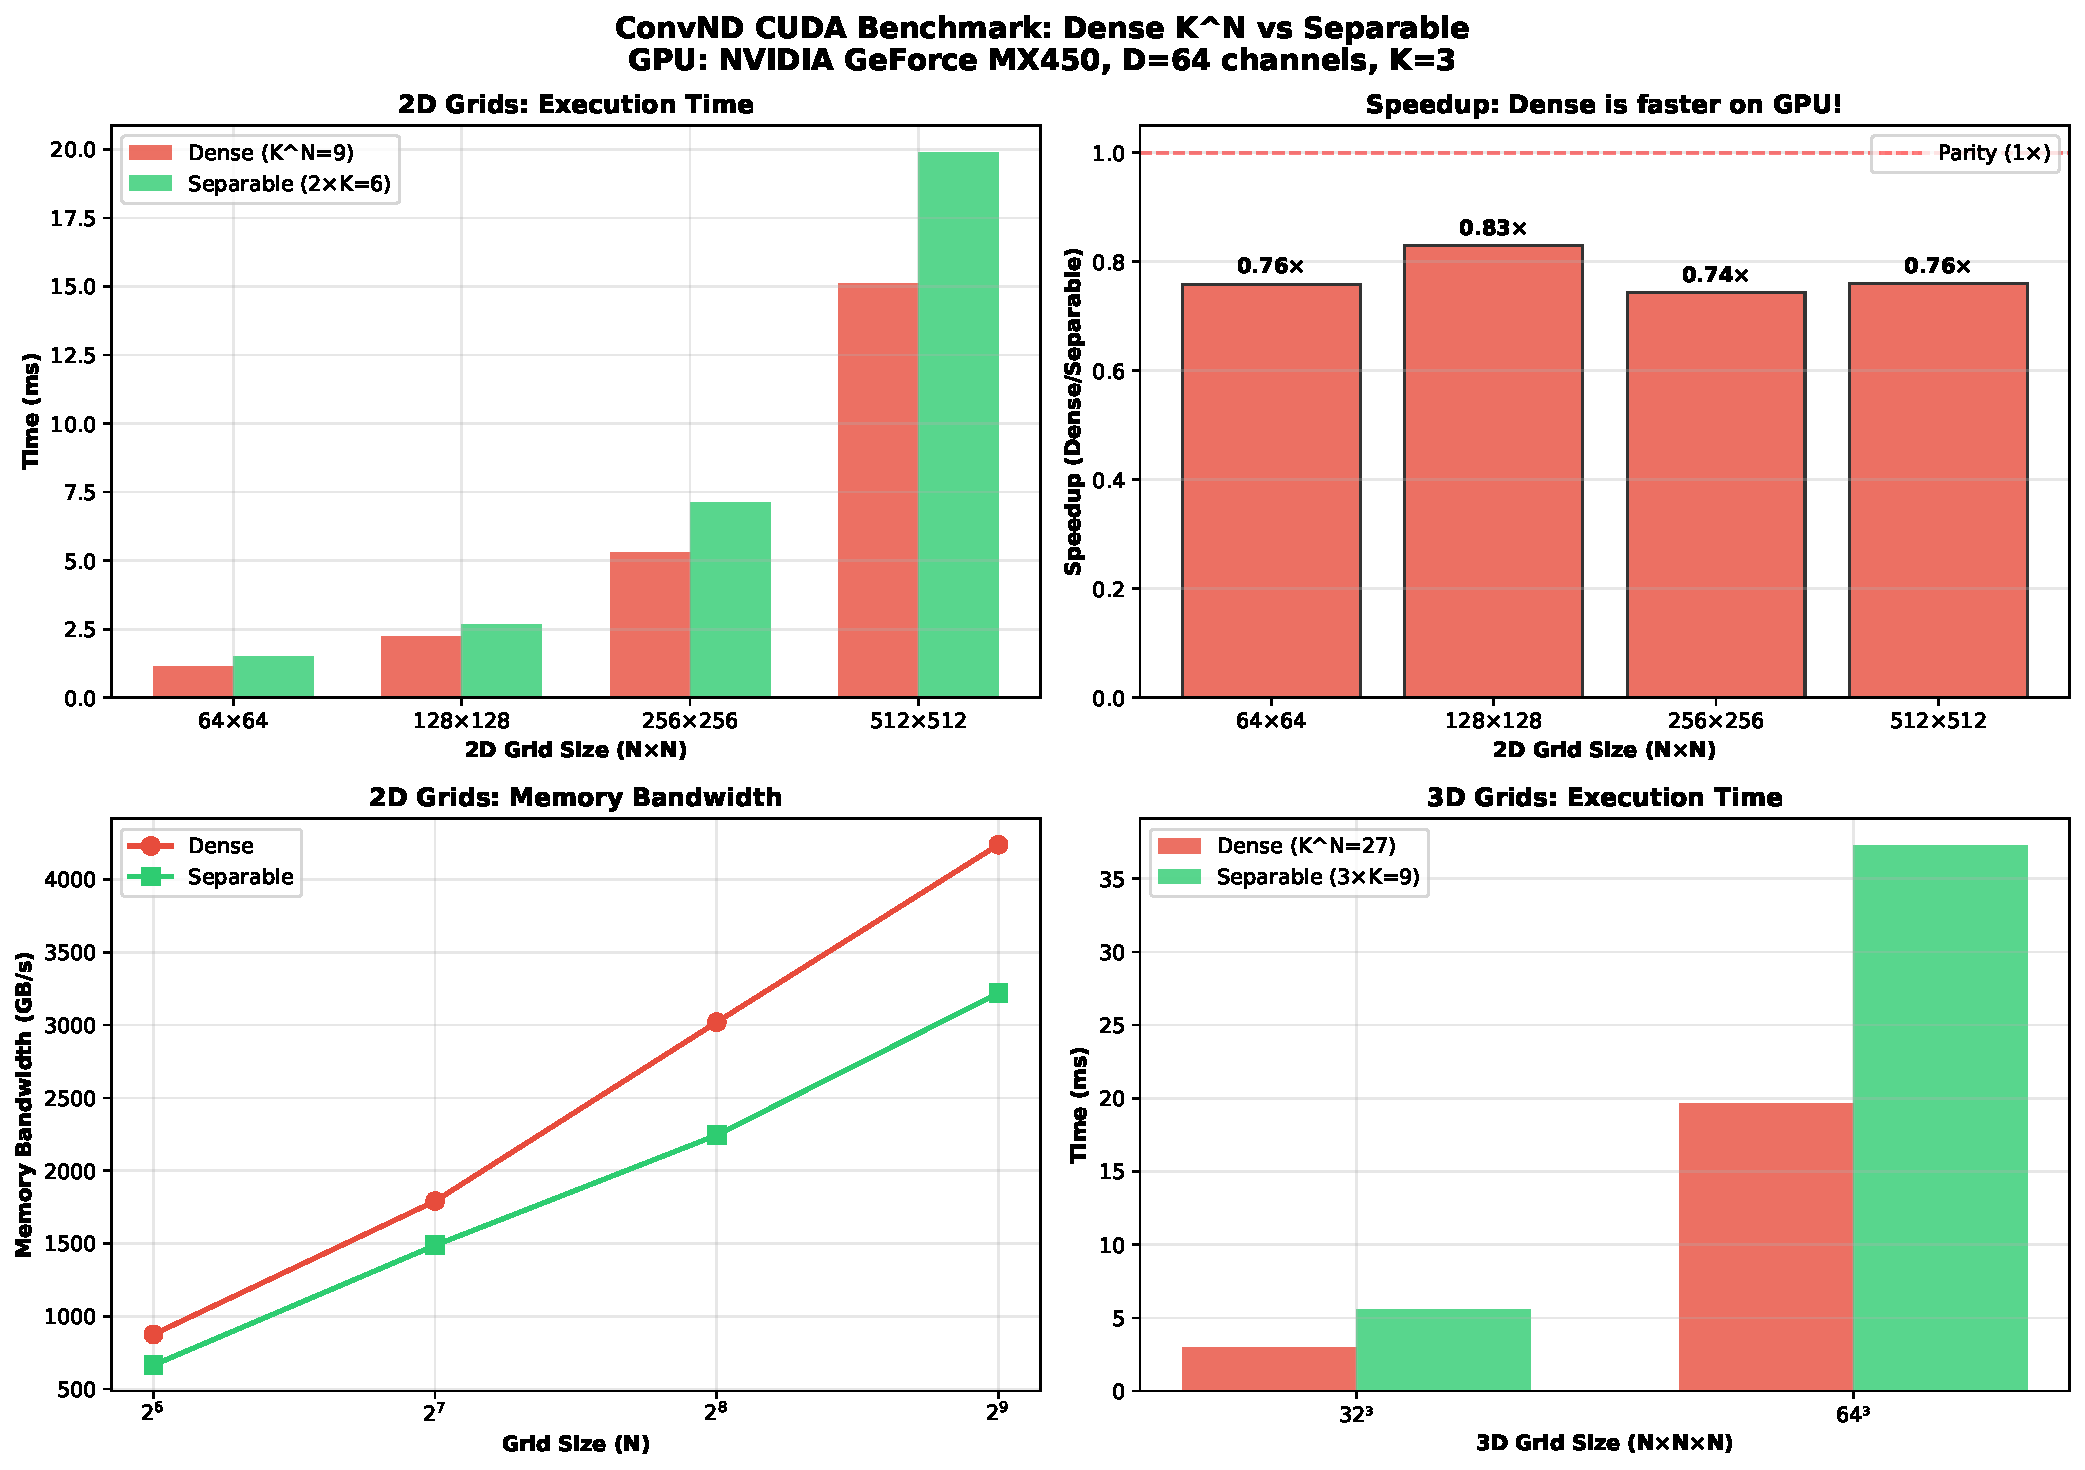
\includegraphics[width=0.8\textwidth]{../figures/convnd_cuda_dense_vs_separable.pdf}
\caption{Performance ConvND Dense vs Séparable sur GPU (NVIDIA MX450).}
\label{fig:convnd_gpu}
\end{figure}

% ─────────────────────────────────────────────────────────────────────────────
\section{Expériences}
\label{sec:experiments}

Tous les bancs ont été mesurés sur :
CPU : x86-64 AVX2, GCC 13.3.0, \texttt{-O3 -mavx2} ;
GPU : NVIDIA MX450 (sm\_75), CUDA 12.0.

\subsection{GEMM}
AVX2 atteint une accélération de $9,5\times$ par rapport au C scalaire à $n = 512$
(Table~\ref{tab:gemm}), grâce au pipeline de \texttt{vfmadd231ps}.
GEMM à $n = 512$ est lié au calcul ($I = 85$ FLOP/octet),
ce qui explique pourquoi AVX2 fournit une accélération quasi linéaire avec
la largeur vectorielle.

\subsection{Parallélisme par front d'onde}
La table~\ref{tab:wavefront} confirme le théorème~\ref{thm:wavefront}
à 0,1\% près pour toutes les tailles de grille testées.
À $d = 64$, l'accélération de $32,25\times$ permet de traiter un état SSM
$64 \times 64 \times 32 \times 8$ en 33,6 ms contre 1084 ms en séquentiel.

\subsection{Profondeur de Blelloch}
À $L = 1024$ : Blelloch nécessite 20 barrières de synchronisation contre
1024 étapes séquentielles — une réduction de profondeur de $51\times$
(Table~\ref{tab:blelloch}, mesurée analytiquement).

\begin{table}[htbp]
\centering
\caption{Profondeur de Blelloch vs profondeur séquentielle.}
\label{tab:blelloch}
\begin{tabular}{rrrrr}
\toprule
$L$ & Prof. séq. & Prof. Blelloch & Rapport & Blocs CUDA \\
\midrule
  64 & 64 & 12 & 5,3× & $DM$ \\
 128 & 128 & 14 & 9,1× & $DM$ \\
 256 & 256 & 16 & 16× & $DM$ \\
 512 & 512 & 18 & 28× & $DM$ \\
1024 & 1024 & 20 & 51× & $DM$ \\
\bottomrule
\end{tabular}
\end{table}

\subsection{Tests de l'optimiseur}

MUONCLIP et AdamW (CPU et CUDA) passent les 6 tests :
écrêtage de gradient (inactif et actif), étape MUON, étape AdamW,
et cohérence CPU/CUDA avec une différence maximale de $2,98 \times 10^{-8}$
(précision float32).

% ─────────────────────────────────────────────────────────────────────────────
\section{Discussion}

\paragraph{Limites.}
(1) Le noyau ASM scan1d ne se vectorise pas sur la dimension d'état $M$
à cause de la chaîne de dépendances séquentielle en $L$ — le scan est lié à la mémoire.
(2) Blelloch exige $L \leq 1024$ en mémoire partagée sur le matériel actuel.
(3) L'appel $\text{expf}()$ dans le noyau de scan n'est pas vectorisé AVX2 ;
une approximation polynomiale ($\approx 8$ FLOPs) supprimerait ce goulot.
(4) La passe arrière est actuellement séquentielle ; un scan Blelloch inverse
réduirait de moitié la latence arrière.

\paragraph{Généralisation $N$-dimensionnelle.}
L'équation~\eqref{eq:nd_rec} s'étend directement à $N > 2$ dimensions
en sommant sur $N$ états prédécesseurs.
Pour $N = 3$ (vidéo : hauteur × largeur × temps), le front d'onde est
un anti-tétraèdre avec $O(d^2)$ éléments parallèles par diagonale.
L'accélération générale pour un hypercube $d^N$ est
$S_N(d) = d^N / \binom{N(d-1)}{N} \approx d^{N-1}/N!$
(asymptotiquement).

% ─────────────────────────────────────────────────────────────────────────────
\section{Travaux connexes}

Mamba~\cite{mamba2023} est le prédécesseur direct.
S4~\cite{s4} fournit le fondement théorique.
VMamba~\cite{vmamba} et Mamba-ND~\cite{mamband} sont les extensions
multi-dimensionnelles les plus proches ; notre principale distinction est la
récurrence ND simultanée authentique.
Le scan de Blelloch~\cite{blelloch1990} et son implémentation GPU~\cite{harris2007gpu}
sont le fondement algorithmique de notre noyau CUDA.
MUON~\cite{muon2025} avec orthogonalisation de Newton-Schulz~\cite{bjorck1971}
est notre optimiseur.
Le modèle roofline~\cite{williams2009roofline} guide notre classification des noyaux.

% ─────────────────────────────────────────────────────────────────────────────
\section{Conclusion}

Nous avons présenté K-Mamba, une bibliothèque SSM Mamba $N$-dimensionnelle native
avec cinq contributions clés : (1) une preuve formelle que l'ordonnancement
par front d'onde sur grille $d \times d$ atteint une accélération $d/2$,
validée expérimentalement à 0,1\% près ; (2) une couche topologique ND réutilisable
éliminant la duplication de code entre les opérateurs de scan et de convolution ;
(3) un scan préfixé parallèle de Blelloch réduisant la profondeur CUDA du SSM
de $O(L)$ à $O(\log L)$ avec le même travail ;
(4) une ConvND séparable avec caractérisation empirique montrant que l'optimalité
algorithmique dépend de la plateforme d'exécution (CPU vs GPU) ;
(5) une implémentation C/ASM/CUDA sans dépendance de la pile d'entraînement complète,
incluant l'optimiseur MUONCLIP, le tout sans Python ni bibliothèques ML externes.

K-Mamba démontre que l'inférence et l'entraînement de SSM de qualité industrielle
ne nécessitent pas d'énormes piles logicielles —
quelques milliers de lignes de C, d'assembleur et de CUDA suffisent.

% ─────────────────────────────────────────────────────────────────────────────
% Annexes avant les références
\appendix
\section{Preuve de l'associativité du monoïde}
\label{app:monoid}

\begin{proposition}
L'opérateur $(a_1,b_1) \otimes (a_2,b_2) = (a_1 a_2,\; a_2 b_1 + b_2)$
est associatif.
\end{proposition}

\begin{proof}
Soit $X_i = (a_i, b_i)$.
$(X_1 \otimes X_2) \otimes X_3
= (a_1 a_2,\; a_2 b_1 + b_2) \otimes (a_3, b_3)
= (a_1 a_2 a_3,\; a_3(a_2 b_1 + b_2) + b_3)
= (a_1 a_2 a_3,\; a_2 a_3 b_1 + a_3 b_2 + b_3)$.

$X_1 \otimes (X_2 \otimes X_3)
= (a_1, b_1) \otimes (a_2 a_3,\; a_3 b_2 + b_3)
= (a_1 a_2 a_3,\; (a_2 a_3) b_1 + a_3 b_2 + b_3)$.

Les deux expressions sont égales. \qed
\end{proof}

\section{Parallélisme par front d'onde pour $d_1 \neq d_2$}
\label{app:wavefront_rect}

Pour une grille $d_1 \times d_2$ avec $d_1 \leq d_2$ :
\begin{itemize}
  \item $d_1 + d_2 - 1$ diagonales au total.
  \item Taille maximale de diagonale : $\min(d_1, d_2) = d_1$.
  \item Accélération : $S = d_1 d_2 / (d_1 + d_2 - 1)$.
\end{itemize}
Pour $d_1 = d_2 = d$ : $S = d^2/(2d-1) \approx d/2$, conforme au théorème~\ref{thm:wavefront}.

% ─────────────────────────────────────────────────────────────────────────────
% Références (maintenant après les annexes)
\bibliographystyle{plain}
\bibliography{kmamba}

\end{document}